% 
% Annual Cognitive Science Conference
% Sample LaTeX Paper -- Proceedings Format
% 

% Original : Ashwin Ram (ashwin@cc.gatech.edu)       04/01/1994
% Modified : Johanna Moore (jmoore@cs.pitt.edu)      03/17/1995
% Modified : David Noelle (noelle@ucsd.edu)          03/15/1996
% Modified : Pat Langley (langley@cs.stanford.edu)   01/26/1997
% Latex2e corrections by Ramin Charles Nakisa        01/28/1997 
% Modified : Tina Eliassi-Rad (eliassi@cs.wisc.edu)  01/31/1998
% Modified : Trisha Yannuzzi (trisha@ircs.upenn.edu) 12/28/1999 (in process)
% Modified : Mary Ellen Foster (M.E.Foster@ed.ac.uk) 12/11/2000
% Modified : Ken Forbus                              01/23/2004
% Modified : Eli M. Silk (esilk@pitt.edu)            05/24/2005
% Modified : Niels Taatgen (taatgen@cmu.edu)         10/24/2006
% Modified : David Noelle (dnoelle@ucmerced.edu)     11/19/2014

%% Change "letterpaper" in the following line to "a4paper" if you must.

\documentclass[10pt,letterpaper]{article}

\usepackage{hyperref}
\usepackage{cogsci}
\usepackage{pslatex}
\usepackage{amsfonts}
\usepackage{graphicx}
\usepackage{apacite}
\usepackage{color}
\usepackage{todonotes}

\definecolor{Red}{RGB}{255,0,0}
\newcommand{\red}[1]{\textcolor{Red}{#1}}

\newcommand{\jd}[1]{\green{$^*$}\marginpar{\footnotesize{JD: \green{#1}}}}

\newcommand{\subsubsubsection}[1]{{\em #1}}
\newcommand{\eref}[1]{(\ref{#1})}
\newcommand{\tableref}[1]{Table \ref{#1}}
\newcommand{\figref}[1]{Figure \ref{#1}}
\newcommand{\appref}[1]{Appendix \ref{#1}}
\newcommand{\sectionref}[1]{Section \ref{#1}}

\title{Why do you ask? To be informative.}
 
\author{{\large \bf Robert X.~D.~Hawkins (rxdh@stanford.edu)} \AND {\large \bf Andreas Stuhlm\"uller (andreas@stuhlmueller.org)}\\ 
	\AND
	{\large \bf Judith Degen (jdegen@stanford.edu)} 
  \AND {\large \bf Noah D.~Goodman (ngoodman@stanford.edu)} \\
  Department of Psychology, 450 Serra Mall \\
  Stanford, CA 94305 USA}


\begin{document}

\maketitle


\begin{abstract}


\textbf{Keywords:} 
questions; answers; computational pragmatics; theory of mind; 
\end{abstract}

\section{Introduction}
\label{sec:intro}

% TODO:
% * refine example in intro paragraph -- something that better emphasizes 'question-as-signal'
% * design evocative cartoon for first page?
% * computational experiments, and transition into behavioral experiment
% * incorporate discussion of model fitting 
% * include rigorous model comparison tests in results 
% *** (can we rule our the pragmatic questioner on the basis of model complexity?)
% * figure out whether related work section is worth the space, or if we want to factor into intro
% * expand discussion to include the limitations of our experiment
Suppose your friend asks you, ``Who is coming to the concert tonight?'' How do you respond? You certainly don't need to give the full list of attendees -- most of whom you do not know -- even though they would all technically be valid answers. Instead, you might only mention the set of \emph{mutual acquaintances} you know are planning to come, assuming that your friend doesn't care about the rest of the crowd. Now, imagine a different scenario. Suppose that you're waiting in line at the box office and want to find out whether your acquaintances had tickets as well. What question would you ask to the person in the ticket booth? If you asked, ``Who is coming to the concert tonight?''  you would likely get a quizzical look and an answer like ``A lot of people, why?'' because the person at the booth does not know your friends or your reason for asking the question. Instead, you might have to directly ask about your friends. Whether you're asking or answering questions, you must engage in some reasoning about the other person's intentions and knowledge. 

Since both questioners and answerers appear to be acutely sensitive to one another's intentions and knowledge, what makes a question useful? What makes an answer to a question useful? In this paper, we present three progressively more sophisticated computational models of question-answer behavior, which formalize and probe this deep interaction between the way answerers infer intentions and the way questioners signal them. We compare these models on the basis of two simulations of classic question-answer phenomena and one experiment in which participants must ask and answer questions given a fixed set of goals. We find that a sophisticated pragmatic answerer is needed to account for the data, and close by proposing that the purpose of questions in dialogue is to provide cues to the answerer about the questioner's goals and intentions.

A number of studies in psycholinguistics have provided evidence that answerers are both sensitive to a questioner's goals and attempt to be informative with respect to those goals. For example, when people are asked `Do you have the time?'' they typically round their answers to the nearest 5 or 10 minute interval, even when they're wearing a digital watch \cite{DerHenstCarlesSperber02_RelevanceTellingTime}. However, if the question is preceded by the statement ``My watch stopped,'' people make their response precise to the minute  \cite{GibbsBryant08_OptimalRelevance}. While an approximate time is sufficiently informative with respect to most goals, like making it to a meeting on time, this experiment demonstrated that answerers were able to infer that the goal of setting a watch required more precise information.

Similar evidence comes from a classic study where researchers called liquor merchants and opened the conversation with one of two sentences: "I want to buy some bourbon'' (the `uninformative' condition) or ``I've got \$5 to spend'' (the `literal' condition) They then asked, ``Does a fifth of Jim Beam cost more than \$5?'' Merchants gave an exact price significantly more often in the `uninformative' context than the `literal' context, where a `yes' or `no' answer was more common. In the former case, the merchant inferred that the questioner's goal was just to buy whiskey, so the exact price was the maximally relevant response. In the latter case, the merchant inferred that the questioner's goal was literally to find out whether or not they could afford the whiskey, hence a simple `yes'  sufficed \cite{Clark79_IndirectSpeechActs}. Context and questioner goals have also been implicated in accounts of identification questions like ``who is X?'' \cite{BoerLycan75_KnowingWho}, and to questions like ``where are you?'' that permit answers at many levels of abstraction \cite{Potts12_CardsDialogueCorpus}. While most of this work has focused on \emph{answerer} behavior, it suggests that the question itself can signal the questioner's goals.

% I think we need to discuss at least one previous model, to make it clear why the problem we're tackling is a problem in the first place. The rest can be in related work at the end.
Recent formal models of question-answer pragmatics have made progress by formally specifying the questioner's goals and what it means for an answerer to be informative with respect to them. van Rooy \citeyear{VanRooy03_QuestioningDecisionProblems}, for instance, defines a goal as a utility function defining a decision problem faced by the questioner. A useful answer under this decision theoretic account is one that maximizes the expected value of the questioner's utility by reducing their uncertainty about the true state of the world. A useful question is one that allows for a sufficiently fine-grained set of answers, optimally distinguishing the worlds relevant to their decision problem. While this framework elegantly accounts for the context-dependence and relevance-maximization of question and answer behavior, it assumes that the questioner's decision problem is known \emph{a priori} by the answerer or fully determined by context. This minimizes the role of the questioner; they just establish a space of answers and then let the answerer do the rest of the work. If the answerer is so adept at using context to determine the relevant information, though, why does the questioner need to ask a question in the first place? Is it just a formality, to prompt the other for their information, or does it serve as a signal in itself, as the studies above suggest? 

We claim that the questioner must reason about answerer behavior, in order to determine what question will produce the most useful answers. This raises a further issue: what kind of answerer does the questioner reason about, and is this internal model accurate? The rest of this paper is structured as follows. First, we specify a family of questioner and answerer agents extending the Rational Speech Act (RSA) framework \cite{frank2012, GoodmanStuhlmuller13_KnowledgeImplicature}, highlighting some points of divergence from previous RSA models. We then individuate three particular models in this family, representing progressively more sophisticated hypotheses about how questioners and answerers reason about their task. In particular, we compare a pragmatic answerer making inferences about the questioner's goals to two simpler models: one that takes into account only that an answerer wants to be maximally informative with respect to the explicit question asked (without inferring the questioner's underlying decision problem) and one that provides a literal answer to the question (without attempting to be maximally informative).  

To compare these models, we derive predictions for a pair of experiments using a novel guessing-game task, and compare these predictions to human performance. In one phase of the task, we require participants to ask a question (from a fixed set of possible questions), given a decision problem. In the second phase, we require participants to give an answer (from a fixed set of possible answers) to a question (from a fixed set of possible questions). These models and data, combined with the psycholinguistic data above, seeks to place question-answer behavior in the larger class of social behavior governed by theory of mind.

\section{A Rational Speech Act model of question and answer behavior}
\label{sec:model}

Suppose there is a set of distinct world states $\mathcal{W}$, a set of possible goals $\mathcal{G}$, a set of possible questions $\mathcal{Q}$, and a set of possible answers $\mathcal{A}$. These sets are all taken to be in common ground between two participants in a dialogue, whom we call the questioner and the answerer. We begin by thinking about how an optimal questioner should choose a question. Critically, instead of trying to impart information about the state of the world, a questioner attempts to \emph{learn information about a private goal}, sometimes called a QUD (or question under discussion) \cite{Roberts96_InformationStructureDiscourse}. A goal $g \in \mathcal{G}$ is a projection function that maps a complete world state to a particular feature or set of features that the questioner cares about. Each of these projections corresponds to a different utility function, in a decision-theoretic formulation. In order to learn information about their private goal $g$, the questioner reasons about how an internal model of an answerer would respond given some true world. 

\begin{itemize}

\item The \textbf{questioner} takes a goal $g \in \mathcal{G}$ as input and returns a distribution over questions $\mathcal{Q}$. To do this, it first computes a prior $P_g(w)$ over the features of the world relevant to its goal. For each question $q \in \mathcal{Q}$, it computes the expected information gain, averaged over all possible true worlds, and all possible responses the answerer could give. Information gain is measured as the  Kullback-Leibler divergence between the prior distribution and the posterior distribution over world states after hearing the answerer's (hypothetical) response: $$P(q | g) \propto \sum_{a \in \mathcal{A}} \sum_{w^* \in \mathcal{W}} P(w^*) P(a | q, w^*) D_{KL}(P_g(w)\, \| \, P_g(w | q, a))$$ 

\end{itemize}

First, note that the questioner depends on $P_g(w | q, a)$, an `interpreter' function that gives the likelihood of different worlds given question and answer pairs. We will specify this function later. Second, and more critically, the questioner depends critically on the answer distribution $P(a | q, w^*)$, which it uses to upweight questions $q$ that elicit useful answers across different world $w^*$ and downweight questions that elicit vague or irrelevant answers. We now propose three different answerer agents that embody different assumptions that the questioner could make.

\begin{itemize}

\item The \textbf{literal answerer} takes a question utterance $q \in \mathcal{Q}$ and a true world state $w \in \mathcal{W}$ as input and returns a distribution over the answer space $\mathcal{A}$. It samples an answer  $a$ from $\mathcal{A}$ with prior probability $P(a)$ and conditions on the likelihood of the questioner inferring the true world $w$ from this answer, using only the interpreter function as a cue. Note that this agent ignores the question; its only concern is to convey the true state of the world. This makes it equivalent to the speaker in previous RSA models.
$$P(a | q,w^*) \propto P(w = w^* | q, a) P(a) $$
\item The \textbf{explicit answerer} samples an answer $a$ from $\mathcal{A}$ with prior probability $P(a)$, then uses the explicit utterance $q$ as a QUD when evaluating the likelihood of a world under an interpreter. 
$$P(a | q, w^*) \propto P_q(w= w^* | q, a) P(a)$$
The only difference here is the projection $q$ it applies to the interpreter output. 
\item The \textbf{pragmatic answerer} uses an internal model of the explicit questioner (i.e. the questioner who reasons about an explicit answerer) as a generative model of questions given goals in order to estimate the likelihood of different goals given the question $q$. It samples an answer $a$ from $\mathcal{A}$ with prior probability $P(a)$, uses the internal questioner model to estimate the likelihood of different goals $g \in \mathcal{G}$ given their question $q$, and attempts to be informative with respect to this goal:
$$\begin{array}{rcl}
P(a | q, w^*) & \propto & P(g | q)  \times P_g(w = w^* | q, a) \times P(a)\\
                    & \propto & P(q | g)P(g) \times P_g(w = w^* | q, a)  \times P(a)\\
\end{array}$$
\end{itemize}

Finally, we must define the interpreter function that all of these agents are using to compute the likelihood of a world given a question and an answer. This is where we specify semantic assumptions about the meaning of a question and answer. For the purposes of this paper, we will use Groenendijk \& Stokhof semantics \citeyear{GroenendijkStokhof84_SemanticsOfQuestions}, where a question induces a partition $\mathcal{P}_q$ over the space of possible world and each cell�of this partition is an equivalence class corresponding to a different answer. An answer, then, selects a cell of this partition, denoted by $\mathcal{P}_q(a)$, which is a set.

\begin{itemize}
\item The \textbf{interpreter} takes a question $q$ and an answer $a$ and returns a distribution of worlds that are consistent with this pair:

$$P(w | q, a) = P(w) \mathbb{I}_{\mathcal{P}_q(a)}(w)$$

where $\mathbb{I}_A(w)$ is the indicator function returning 1 if $w \in A$ and 0 otherwise.
\end{itemize}
This concludes our specification of the model space, giving a set of three answerers and three corresponding questioners that reason about them. Within this computational framework, different theories of question and answer behavior can be formalized and compared on the basis of their predictions. Assumptions about what is held in common ground are made transparent, and we can systematically manipulate individual elements of the model to test how they affect overall predictions. Because these are probabilistic models, we can succinctly write them down and evaluate their predictions in a probabilistic programming language \cite{Goodman13_POPL}. The model predictions shown throughout the rest of the paper were computed using a language called WebPPL \cite{GoodmanStuhlmuller14_DIPPL}. Note that this specification diverges from previous work in the RSA framework in a few key ways: (1) for the questioner, we replace the goal of imparting information with the goal of learning information about the specified QUD and (2) \dots \todo[inline]{RDH: any other major differences?}

\section{Simulations}

Before presenting our experimental paradigm, we present two computational simulations demonstrating the way our model captures some classic psycholinguistic phenomena. Because the most well-studied phenomena are primarily about the \emph{answerer}'s sensitivity to goals, these simulations cannot demonstrate the full contribution our model makes toward understanding questioner behavior -- if there is only one question, it does not serve as a signal -- but we include them with the intention of providing some context for our later results. In the first case, we show how the questioner's prior affects the pragmatic answerer, and in the second, we show how a piece of context supplied by the questioner can change the pragmatic answerer's response. 

\subsection{`Mention-some' questions}

\emph{wh}-questions admit two interpretations: `mention-all' and `mention-some.' If a doctor walks into a clinic and asks `who is sick?' this likely means that they want to know, of \emph{each} person in the clinic, whether or not they are sick. This is a `mention-all' interpretation. If they ask `where can I buy a newspaper?', however, this likely means they only want to know one or two particularly good places. This is a `mention-some' interpretation. There is a long tradition of refinements and solutions to the problem of which questions admit which kind of answers in theoretical linguistics \cite<see>{George11_Dissertation}. We present a highly simplified account of answers to the question ``Who was at the party?'' 

\todo[inline]{RDH: could also do `newspaper.' Also, don't need as much detail I give in the following \P...}
Suppose there are four people in the universe, and each person was either at the party or not. The world space $\mathcal{W}$ contains all $2^4 = 16$ possible assignments of the four people to booleans. There is only one question: $\mathcal{Q} =$ ``who was at the party?'', but $15$ underlying goals in $\mathcal{G}$: they might be interested in knowing about any combination of one or more people: the power set over the four people. The answerer can tell the questioner about any subset, so the answer space $\mathcal{A}$ is also a power set. Our agents are set up exactly as specified in the previous section, with some additional assumptions made about their prior distributions. In particular, we put a generic cost on longer utterances, consistent with previous empirical work (cite XXX).

To test whether a `mention-some' interpretation can arise from sensitivity to a questioner's goals, we gave the questioner agent a goal prior $P(g)$ with higher probability assigned to some people than others. The likelihood of sets containing multiple individuals was simply the product of the probabilities assigned to individuals in the set. Due to the utterance length cost, the explicit answerer did prefer mentioning `some' than `all' but demonstrated no sensitivity to which individuals the questioner cared about more. Since there was no information in the signal, the pragmatic answerer had to rely solely on the goal prior $P(g)$ to choose its response and therefore trivially matched the questioner's preferences.

To test a `mention-all' interpretation, we kept the utterance length cost in place, but shifted the questioner's goal prior to place priority on the maximal set. This captures, for example, the doctor's interest in all his or her patients collectively. Under this new goal prior, the explicit answerer shows no difference in behavior, because the explicit question being asked was fixed. But, as expected, the pragmatic answerer overcomes their intrinsic bias toward short utterances and prefers to be informative with respect to the full group of people the questioner was interested in.

\todo[inline]{RDH: I don't know how much the preceding really tells us about q\& a behavior, or our model\dots if all we have to say is ``the mention-some/mention-all distinction arises from different priors,'' we're (a) over-simplifying the linguistic literature on this, and (b) saying that the pragmatic answerer knows ahead of time what the questioner cares about \dots}

\subsection{Whiskey pricing}

Next, we show that our model can reproduce the behavior found by Clark \citeyear{Clark79_IndirectSpeechActs}, who demonstrated that context providing indirect evidence for a questioner goal can shift answerer behavior \dots

\section{Experiment 1: \\ Questions and answers in a hierarchical world}

\todo[inline]{RDH: Pivot here}
	While there is extensive evidence that answerers are sensitive to questioner goals and context, the novel prediction of our model is about \emph{questioner behavior}. If the pragmatic answerer uses the question itself as a signal about which underlying goal is currently at play, the questioner should choose questions that make their underlying intentions most clear.  In order to test how questioners choose questions when given a decision problem, and how answerers choose answers under uncertainty about this decision problem, we designed a guessing-game task played by two players: a guesser (the questioner) and a helper (the answerer). In this game, $4$ animals (a dalmatian, a poodle, a siamese cat, and a goldfish) were hidden behind $4$ gates. Note that these animals correspond to different levels in a class hierarchy (see Fig. \ref{fig:taskhierarchy}). The guesser was given a private goal of finding one of the objects (e.g. `find the poodle'), and the helper had privileged information about the exact locations of each object. Before choosing a gate, the guesser could ask the helper a single question, chosen from a restricted set of options, and the helper could respond to this question by revealing the object behind a single gate. 

In terms of our model specification, the world space $\mathcal{W}$ is the set of $4! = 24$ possible assignments of four objects to four gates and the goal space $\mathcal{G}$ is the set of four objects that the guesser could possibly be trying to find, and the answer space $\mathcal{A}$ is the set of four gates that the helper could possibly reveal. The key constraint in the task, however, is that the guesser must choose from a \emph{restricted set of questions}: they may be trying to find the goldfish, but cannot directly ask `where is the goldfish?' Instead, the question space $\mathcal{Q}$ is the set of highlighted nodes in the hierarchy, including higher order nodes that are consistent with multiple answers. 

\begin{figure}
\begin{center}
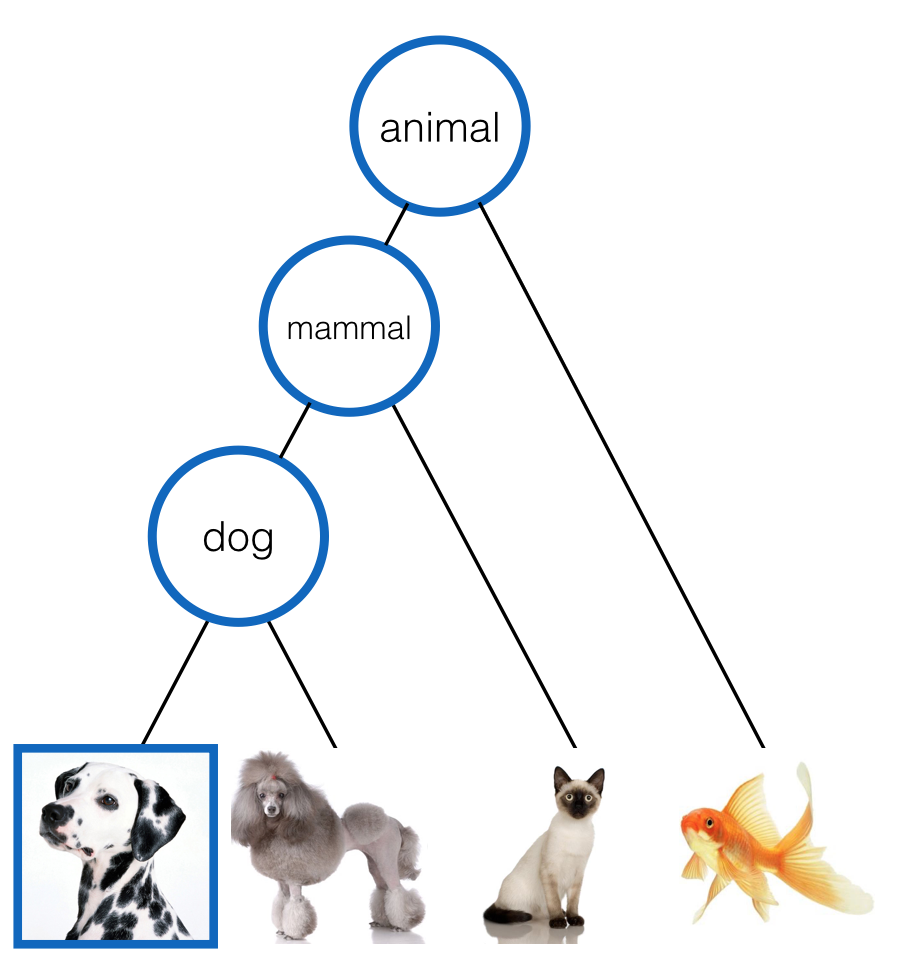
\includegraphics[scale = .4]{taskhierarchy}
\end{center}
\caption{Stimulus hierarchy used in experiment 1. The goal space and answer space contained the four object hidden behind gates (the nodes of the tree). The question space, however, was restricted to the highlighted nodes, proceeding up the hierarchy. This allows us to test the extent to which the answerer infers questioner goals. For example, both the dalmatian and poodle would be truthful responses to the explicit question `dog?' but only one is the true goal.}
\label{fig:taskhierarchy}
\end{figure}


We recruited 25 participants from Amazon Mechanical Turk to participate in this task. Each participant provided responses for four trials in the role of the questioner (corresponding to each goal in $\mathcal{G}$), and four trials in the role of the answerer (corresponding to each question in $\mathcal{Q}$). In order to collect responses for all elements of $\mathcal{G}$ and $\mathcal{Q}$, the order of� the questioner and answerer blocks was randomly assigned, and the order of stimuli within these blocks was also randomized\footnote{All materials are available at \url{https://github.com/hawkrobe/Q\_and\_A/tree/master/experiment3/versions/experiment3\_short}}. Two participants were excluded due to self-reported confusion about the task.

Results for the guesser role are shown with our model predictions in Figure \ref{fig:exp1res}(a). There are two primary trends to note in these data. First, questioners do prefer to ask different questions given different goals, even as those questions become less explicitly informative. \todo[inline]{stats} We observe that participants prefer indirect question node closest to their goal when the direct question is unavailable. It is unsurprising that they ask about the `dalmatian` when looking for the dalmatian, but interesting that they strongly prefer asking about a `dog' when looking for the poodle, about a `mammal' when looking for the cat, and so on. Second, the strength with which questioners prefer one question over another decreases as they become more indirect \todo[inline]{stats/explain this better}

\begin{figure*}[t!]
\begin{center}
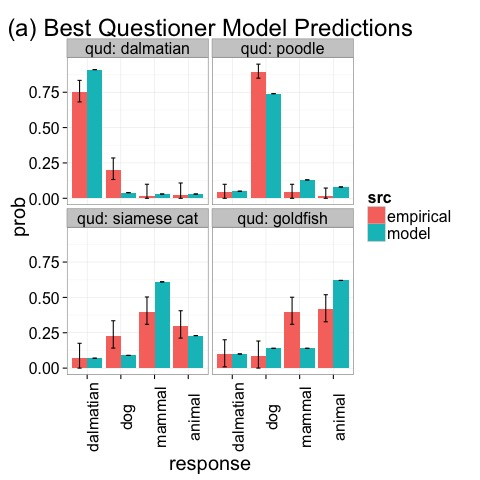
\includegraphics[scale = .52]{questionerDataComparison.jpeg}
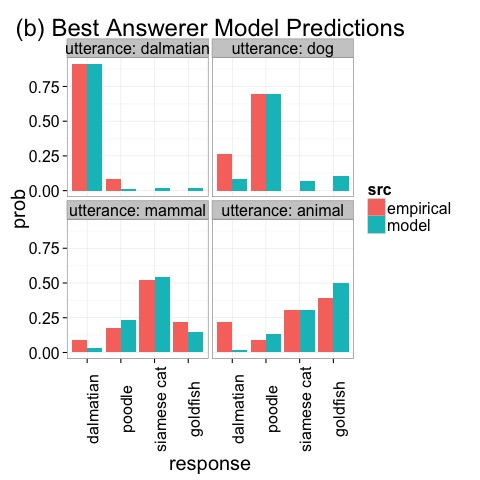
\includegraphics[scale = .52]{answererDataComparison.jpeg}
\end{center}
\caption{These plots show our results from experiment 1, compared with the predictions of our best-performing models for both questioner and answerer behavior. In both cases, the pragmatic agent performed the best. \todo[inline]{RDH: Although, I bet if we actually did a model comparison, the extra .04 correlation you get from going to the pragmatic questioner doesn't justify its complexity\dots which would be a pretty interesting conclusion, actually}}
\label{fig:exp1res}
\end{figure*}
%\label{sec:expq}

Results for the helper role are shown in Figure \ref{fig:exp1res}(b). The most striking feature of these data is how closely the answerer distribution matches the questioner distribution \todo[inline]{RDH: Possibly just because people did both... It might be the second-timers driving the effect, so we should separate out the different orders, or run it again between-subjects} If the helper is asked about a `dog`, the dalmatian and poodle would be equally good literal answers to this question, but they strongly prefer to give the location of the poodle. Similarly, the dalmatian, poodle, and siamese cat are all mammals, but helpers prefer to respond to the `mammal' question by revealing the location of the cat. \todo[inline]{Do a regression here to make this point more rigorously?}


\begin{figure*}[t!]
\begin{center}
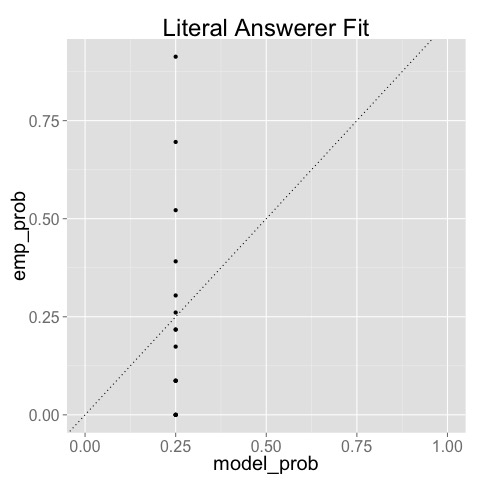
\includegraphics[scale = .33]{bestLitAnswerer.jpeg}
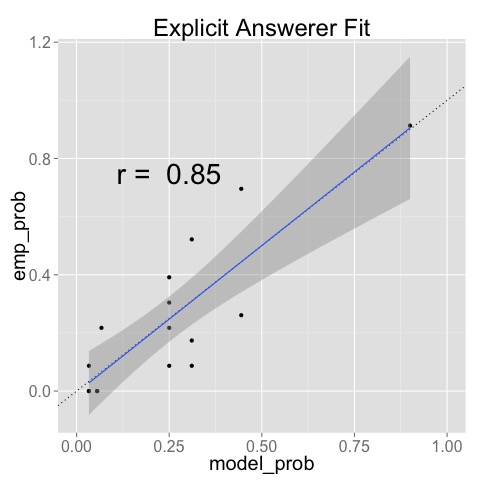
\includegraphics[scale = .33]{bestExpAnswerer.jpeg}
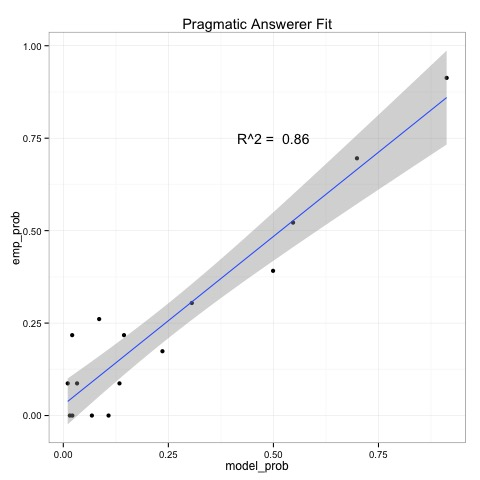
\includegraphics[scale = .33]{bestPragAnswerer.jpeg}

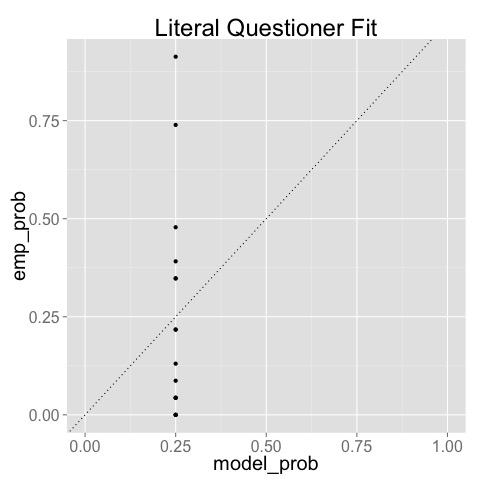
\includegraphics[scale = .33]{bestLitQuestioner.jpeg}
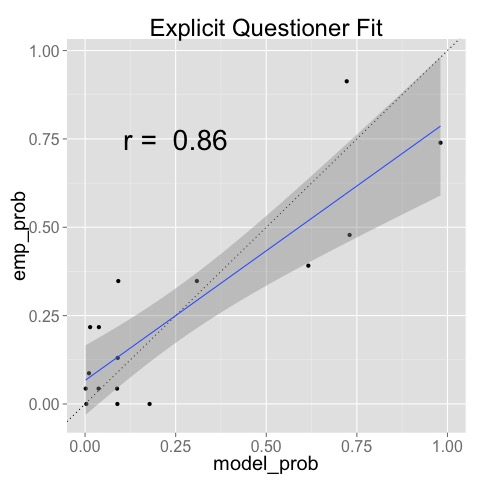
\includegraphics[scale = .33]{bestExpQuestioner.jpeg}
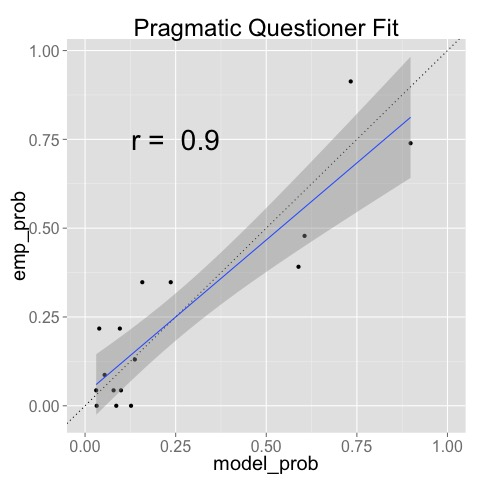
\includegraphics[scale = .33]{bestPragQuestioner.jpeg}
\end{center}
\caption{Full space of models, and their correlations with the data from Experiment 1. The questioner models in the second row reason about the answerers directly above them in the top row, and the pragmatic answerer reasons about the explicit questioner. Note that the explicit answerer model was fit using one rationality parameter, the explicit questioner was fit using two optimality parameters, the pragmatic answerer was fit using four parameters, and these parameters were fixed in the pragmatic questioner \todo[inline]{RDH: There needs to be more discussion of parameter fitting in the body -- the fact that the better models just have more parameters is too easy a target! Maybe if we propagate up the best vals, so that each model only has to fit one or two to its own data?}}
\label{fig:model_space}
\end{figure*}

\subsection{Model comparison}

We now compare these results to the predictions of our family of models (Fig. \ref{fig:model_space}). At the very simplest level, our \emph{literal answerer} yields a uniform distribution over the four answers that are the case in the given world. This has important consequences for the corresponding \emph{literal questioner} model: when this questioner reasons about which question would generate the most helpful answer from the literal answerer, they find no differences, and therefore have no preference over which question to ask. Based on the results presented above, this is clearly not how questioners and answerers behave and we will not consider the literal models further.

At a slightly higher level of sophistication, we have an \emph{explicit answerer}, which is equally likely to give the location of all nodes under the explicit class mentioned in the question (e.g. \emph{dog} or \emph{animal}). This model produces the answerer predictions depicted in Figure \ref{fig:model_space}(b), which successfully down-weights the least relevant alternatives, giving a model-data correlation of $r = 0.85$ \todo[inline]{stats}, with only one free (optimality) parameter, but cannot reproduce some important qualitative symmetries between the explicitly relevant alternatives. For example, it is equally likely to respond `dalmatian' and `poodle' when asked about the `dog', whereas participants significantly preferred `poodle.' The \emph{pragmatic answerer} model, which uses the question utterance to infer the questioner's underlying goal, is able to break this symmetry, for an overall fit of $r = 0.95$ \dots \todo[inline]{depends on how we reuse parameters}

The \emph{explicit questioner}, which reasons about an internal model of an explicit answerer, yields a model-data correlation of $r = 0.86$. If it instead reasons about an internal model of a pragmatic questioner, the fit increases to $r = 0.90$, but the increased model complexity does not justify the improvement in fit  

\section{Related work}

Our account of question and answer behavior ultimately converges on a similar solution as contemporary decision theoretic or game theoretic accounts in linguistics. These theories were a response to early work on question and answer semantics, which focused on the notion of informativeness. In Groenendijk \& Stokhof's \citeyear{GroenendijkStokhof84_SemanticsOfQuestions} theory of question and answer semantics, asking a question induces a partition over the space of possible worlds, where each cell of the partition corresponds to a possible answer. An answer, then, consists of eliminating cells in this partition, and the most useful answers are those that eliminate all relevant alternatives to the true world. However, as van Rooy \cite{VanRooy03_QuestioningDecisionProblems} and others \cite{Ginzburg95_ResolvingQuestions} have pointed out, this predicts that \emph{wh}-questions like ``Where can I buy an Italian newspaper?'' can only be fully resolved by exhaustively mentioning whether or not such a newspaper can be bought at each possible location. Clearly, this is not the case: a single nearby location would suffice. These theories also cannot account for other contextual variation in what counts as a useful answer, such as questions like ``where are you?'' 

% More recent theories have tried to fix these problems by introducing some consideration of the questioner's goals. van Rooy \citeyear{VanRooy03_QuestioningDecisionProblems}, for instance, formalizes these goals as a decision problem faced by the questioner. A useful answer under this decision theoretic account is one that maximizes the expected value of the questioner's decision problem. A useful question is one that induces a sufficiently fine-grained partition, optimally distinguishing the worlds relevant to the decision problem. While this framework elegantly accounts for the context-dependence and relevance-maximization of question and answer behavior, it assumes that the questioner's decision problem is known \emph{a priori} by the answerer. If this were the case, the act of asking questions would seem irrelevant: why wouldn't the answerer directly tell the questioner which action to take? 

\section{General discussion}
\label{sec:gd}

Humans are experts at inferring the intentions of other agents from their actions \cite{TomaselloCarpenter___Moll05_IntentionsCulturalCognition}. Given simple motion cues, for example, we are able to reliably discern high-level goals such as chasing, fighting, courting, or playing \cite{BarrettToddMillerBlythe05_IntentionFromMotionCues, HeiderSimmel44_ApparentBehavior}. Experiments in psycholinguistics have shown that this expertise extends to speech acts as well.  Behind every question lies some goal or intention. This could be an intention to obtain an explicit piece of information (``Where can I get a newspaper?''), signal some common ground (``Did you see the game last night?''), test the answerer's knowledge (``If I add these numbers together, what do I get?''), politely request the audience to take some action (``Could you pass the salt?''), or just to make open-ended small talk (``How was your weekend?''). These wildly different intentions seem to warrant different kinds of answers, even if the explicit question is expressed using the same words.

In this paper we have presented computational-level evidence that answerer behavior is best described by a pragmatic model that reasons about questioner intentions, using the question utterance as a signal. Furthermore, we showed that questioner behavior is best described by a model that reasons about a lower-level explicit answerer. This analysis provides a novel perspective on the role of questions in dialogues: it is well-accepted under the Gricean view that answerers strive to be relevant, but we find that there is also a burden placed on the questioner to provide sufficient information about should be considered relevant in the first place. 

There are some pros and cons to the artificially restricted question space in our experiment design. On one hand, this seems to distance the behavior of participants from the types of questions and answers they would make using natural language. On the other hand, this restriction was crucial in allowing us to compare the informativeness of different questions, serving as a minimal test: when necessary, questioners can choose an optimally informative signal. However, it is worth observing that many conversational scenarios in everyday usage feature natural restrictions on the set of things one can ask about, due to politeness, salience, time cost, and other factors. We must choose our questions carefully. 

\bibliographystyle{apacite}

\setlength{\bibleftmargin}{.125in}
\setlength{\bibindent}{-\bibleftmargin}

\bibliography{bibs}


\end{document}
